\documentclass[zihao=false,fontset=windows]{ctexart}
\usepackage{scrextend}
\changefontsizes[12pt]{10pt}

\usepackage[a4paper,left=2.35cm,right=2.35cm,top=1.7cm,bottom=1.9cm]{geometry}
\usepackage{xcolor}
\usepackage{graphicx}
\usepackage{amsmath,amssymb}
\usepackage{enumitem}
\usepackage{tabularx}
\usepackage{colortbl}
\usepackage{listings}
\usepackage{hyperref}
\usepackage[most]{tcolorbox}

\definecolor{feishuText}{RGB}{31,35,41}
\definecolor{feishuBlue}{RGB}{36,91,219}
\definecolor{feishuRed}{RGB}{216,57,49}
\definecolor{feishuGray}{RGB}{100,106,115}
\definecolor{feishuGray2}{RGB}{143,149,158}
\definecolor{feishuPinkBg}{RGB}{251,191,188}
\definecolor{quoteBar}{RGB}{51,112,255}
\definecolor{codebg}{RGB}{245,246,247}
\definecolor{codeborder}{RGB}{222,224,227}
\definecolor{inlinebg}{RGB}{242,243,245}
\definecolor{callRed}{RGB}{253,226,226}
\definecolor{callOrange}{RGB}{255,245,235}
\definecolor{callYellow}{RGB}{254,255,240}
\definecolor{callGreen}{RGB}{240,251,239}
\definecolor{callBlue}{RGB}{240,244,255}
\definecolor{callRedSoft}{RGB}{254,241,241}
\definecolor{callSun}{RGB}{255,255,204}
\definecolor{cellLilac}{RGB}{246,241,254}
\definecolor{tableHead}{RGB}{242,243,245}
\definecolor{tableRule}{RGB}{222,224,227}
\definecolor{codeText}{RGB}{31,35,41}
\definecolor{codeKeyword}{RGB}{0,0,255}
\definecolor{codeComment}{RGB}{0,128,0}
\definecolor{codeString}{RGB}{163,21,21}

\setmainfont{Times New Roman}
\setCJKmainfont{Microsoft YaHei}[AutoFakeBold=2.2]
\setCJKsansfont{Microsoft YaHei}[AutoFakeBold=2.2]
\setCJKmonofont{Microsoft YaHei}[AutoFakeBold=2.2]
\setmonofont{Consolas}
\newfontfamily\emojifont{Segoe UI Emoji}
\xeCJKsetcharclass{"FE00}{"FE0F}{0}
\xeCJKsetcharclass{"20E3}{"20E3}{0}

\hypersetup{
  colorlinks=true,
  urlcolor=feishuBlue,
  linkcolor=feishuBlue,
  unicode=true,
  pdftitle={CLIP(2021, OpenAI)}
}

\setlength{\parindent}{0pt}
\setlength{\parskip}{0.42em}
\setlength{\fboxsep}{1.5pt}
\setlength{\emergencystretch}{3em}
\linespread{1.28}
\color{feishuText}
\arrayrulecolor{tableRule}
\urlstyle{same}

\setlist[enumerate,1]{label=\textcolor{feishuBlue}{\arabic*.}, leftmargin=1.7em, itemsep=0.22em, topsep=0.28em, parsep=0.08em, partopsep=0pt}
\setlist[enumerate,2]{label=\textcolor{feishuBlue}{\alph*.}, leftmargin=1.8em, itemsep=0.16em, topsep=0.18em, parsep=0.06em, partopsep=0pt}
\setlist[itemize,1]{label=\textcolor{feishuBlue}{\textbullet}, leftmargin=1.35em, itemsep=0.18em, topsep=0.25em, parsep=0.06em, partopsep=0pt}
\setlist[itemize,2]{label=\textcolor{feishuBlue}{◦}, leftmargin=1.45em, itemsep=0.12em, topsep=0.15em}
\setlist[itemize,3]{label=\textcolor{feishuBlue}{\rule[0.18em]{0.38em}{0.38em}}, leftmargin=1.55em, itemsep=0.1em, topsep=0.12em}

\newcommand{\feiEmoji}[1]{{\emojifont #1}}
\newcommand{\incode}[1]{\colorbox{inlinebg}{\ttfamily\small #1}}
\newcommand{\bigmath}[1]{%
  \begin{center}\large$\displaystyle #1$\end{center}%
}

\lstset{
  language=Python,
  basicstyle=\ttfamily\footnotesize\color{codeText},
  keywordstyle=\color{codeKeyword},
  commentstyle=\color{codeComment},
  stringstyle=\color{codeString},
  showstringspaces=false,
  breaklines=true,
  columns=fullflexible,
  keepspaces=true,
  tabsize=4,
  upquote=true,
  aboveskip=2pt,
  belowskip=0pt,
  xleftmargin=0pt,
  frame=none
}
\lstdefinelanguage{clipnp}{
  sensitive=true,
  morecomment=[l]{\#},
  morestring=[b]{'''},
  morestring=[b]{"}
}

\tcbset{
  feishubase/.style 2 args={
    enhanced,
    boxrule=0pt,
    arc=8pt,
    left=10pt,
    right=10pt,
    top=7pt,
    bottom=7pt,
    before skip=6pt,
    after skip=6pt,
    colback=#1,
    colframe=#1,
    before upper={\feiEmoji{#2}\hspace{0.45em}\raggedright\ignorespaces}
  }
}
\newtcolorbox{feishubox}[2]{feishubase={#1}{#2}, breakable}
\newtcolorbox{feishuboxnb}[2]{feishubase={#1}{#2}}

\newtcolorbox{feishuquote}{
  enhanced,
  breakable,
  boxrule=0pt,
  leftrule=3pt,
  arc=0pt,
  colframe=quoteBar,
  colback=white,
  left=8pt,
  right=2pt,
  top=2pt,
  bottom=2pt,
  before skip=4pt,
  after skip=4pt,
  before upper=\color{feishuGray}
}

\newtcolorbox{feishucode}{
  enhanced,
  breakable,
  colback=codebg,
  colframe=codeborder,
  boxrule=0.6pt,
  arc=6pt,
  left=6pt,
  right=6pt,
  top=5pt,
  bottom=4pt,
  before skip=6pt,
  after skip=6pt
}

\begin{document}
{\zihao{1}\bfseries CLIP(2021, OpenAI)\par}
\vspace{0.15em}

\begin{feishuquote}
CLIP：对比学习构建图文桥梁（2021，OpenAI）\par
\href{https://arxiv.org/abs/2103.00020}{Contrastive Language Image Pre-train}\par
\end{feishuquote}
\begin{feishuquote}
多模态，是指不同领域的输入数据，比如文字、图片、语音、视频等等。在传统方法中，每个领域都有一些经典的处理算法，比如用于处理文本的RNN、LSTM、Transformer，用于处理图像的各类CNN等，各领域间相对独立。但是，人们总会遇上需要联合领域数据的时候：比如给一张图片，输出一段关于这个图片的描述；或者给一段文字，输出一张符合文字描述的图片。而实现这一目标的难点在于：不同领域数据间的特征分布、特征信息是不一样的。因此\textbf{多模态模型的总体目标}就是：训练一个模型，一方面能统一特征表达，另一方面又能让不同模态特征间学到相关性。\par
核心任务主要包括表示学习，模态映射，模态对齐，模态融合，协同学习\par
\end{feishuquote}
CLIP模型是一个基于对比文本-图像对的多模态预训练神经网络，由OpenAI于2021年2月提出，能够有效地借助自然语言的监督来学习视觉的概念。CLIP通过跨模态学习，成功地将图像与文本在统一的语义空间中表示，能够让机器同时理解图片和文字，实现图像和文本之间更准确、智能的匹配。\par
\par\vspace{1.15em}\noindent{\zihao{-2}\bfseries 1. CLIP概述}\par\vspace{0.28em}
clip的动机，CV中存在的问题\par
clip的本质，核心\par
\par\vspace{0.75em}\noindent{\zihao{4}\bfseries 1.1 动机}\par\vspace{0.28em}
尽管深度学习在计算机视觉领域带来了革命性的突破，但现有方法仍然面临几个关键问题：\par
\begin{tcbraster}[raster columns=3, raster equal height=rows, raster column skip=9pt, raster row skip=8pt, raster left skip=0pt, raster right skip=0pt]
\begin{feishuboxnb}{callYellow}{1️⃣}
\textbf{数据集构建成本高且覆盖范围有限}\par
典型的视觉数据集往往需要大量人力标注，并且仅涵盖有限的视觉概念，难以扩展到更广泛的场景。\par
\end{feishuboxnb}
\begin{feishuboxnb}{callGreen}{2️⃣}
\textbf{模型泛化能力差，难以适应新任务}\par
传统的视觉模型通常是针对特定任务设计的，若要迁移到新任务，需要额外的微调和大量标注数据。\par
\end{feishuboxnb}
\begin{feishuboxnb}{callBlue}{3️⃣}
\textbf{在现实环境中表现不佳}\par
虽然许多模型在标准基准测试中表现出色，但在压力测试（如应对噪声、遮挡、视角变化等情况下）中的表现往往令人失望。这使得人们对深度学习在计算机视觉中的可行性产生了质疑。\par
\end{feishuboxnb}
\end{tcbraster}
ViT模型在做传统分类任务时，存在两个显著缺点：\par
\begin{enumerate}
\item 如果出现了一张图，其中包含模型从来没见过的类别，那么模型就不能输出正确的结果。
\begin{feishubox}{callOrange}{🌰}
训练时用的是动物图片，预测时却给模型一张汽车图片\par
\end{feishubox}
\item 如果输入数据出现了分布偏移（distribution shift），那么模型可能也无法输出正确的结果。
\end{enumerate}
\begin{feishubox}{callOrange}{🎉}
1中描述的算一种偏移，另外训练时用的是正常的动物图片，预测时给的是毕加索风格的动物图片也算一种偏移\par
\end{feishubox}
解决这2个缺点的传统方法是：\textbf{微调}。但是\textbf{多模态}却想做一步到位的事情：\textcolor{feishuRed}{\textbf{不用做任何微调，也能实现zero-shot的图片分类。}}\par
\begin{feishubox}{callSun}{🌟}
一句话总结clip的论文：\textbf{clip是一个zero-shot的视觉分类模型，预训练的模型在没有微调的情况下在下游任务中获得了很好的迁移效果。}\par
\end{feishubox}
\par\vspace{0.75em}\noindent{\zihao{4}\bfseries 1.2 核心}\par\vspace{0.28em}
\begin{feishubox}{callRed}{❤️}
核心思想：\textbf{对比学习（Contrastive Learning）}，让图像和文字在同一个语义空间中进行对比学习。\par
也可以说是，从自然语言中提取监督信号指导模型学习。\par
CLIP期望通过对比学习，将图像和文本表征映射到一个共同的高维嵌入空间中，使得语义相关的图文对具有较高的相似度，而不相关的图文对相似度较低。\textbf{这样一来，图像和文本虽然来自不同的模态，但它们在共同的语义空间中实现了对齐(alignment)。}\par
\end{feishubox}
\begin{feishuquote}
如果有一张猫咪的照片以及一段描述「一只可爱的猫咪」，CLIP 会学着将这对图片和文字放到相近的位置，同时把不相关的图片-文字对拉远。比如小狗的照片和「一只可爱的猫咪」的描述则会被模型区分开来，放在较远的位置。\par
\end{feishuquote}
这种核心思想的优势：\par
\begin{tcbraster}[raster columns=4, raster equal height=rows, raster column skip=9pt, raster row skip=8pt, raster left skip=0pt, raster right skip=0pt]
\begin{feishuboxnb}{callOrange}{💥}
不需要人工标注，摆脱标签\par
\end{feishuboxnb}
\begin{feishuboxnb}{callOrange}{⛱️}
强大的zero-shot迁移学习能力\par
\end{feishuboxnb}
\begin{feishuboxnb}{callOrange}{🎉}
强大的通用视觉理解能力\par
\end{feishuboxnb}
\begin{feishuboxnb}{callOrange}{🌟}
多模态\par
\end{feishuboxnb}
\end{tcbraster}
\par\vspace{1.15em}\noindent{\zihao{-2}\bfseries 2. CLIP流程}\par\vspace{0.28em}
\begin{center}
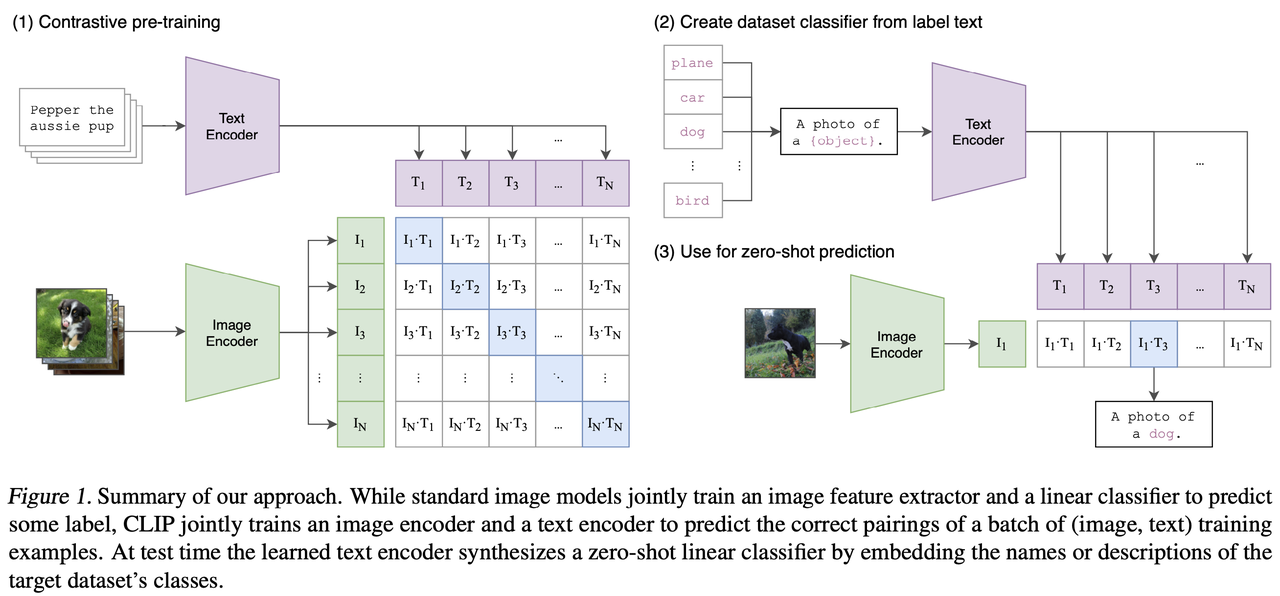
\includegraphics[width=0.98\textwidth]{images/2021-ICML-CLIP/fig-01.png}
\end{center}
\begin{tcbraster}[raster columns=3, raster equal height=rows, raster column skip=9pt, raster row skip=8pt, raster left skip=0pt, raster right skip=0pt]
\begin{feishuboxnb}{callRedSoft}{1️⃣}
\textbf{Contrastive pre-training}：\par
对比预训练阶段，使用image-text对进行对比学习训练。\par
\end{feishuboxnb}
\begin{feishuboxnb}{callRedSoft}{2️⃣}
\textbf{Create dataset classifier from label text}：\par
提取预测类别文本特征。\par
\end{feishuboxnb}
\begin{feishuboxnb}{callRedSoft}{3️⃣}
\textbf{Use for zero-shot prediction}：\par
进行 Zero-Shot 推理预测。\par
\end{feishuboxnb}
\end{tcbraster}
\par\vspace{0.95em}\noindent{\zihao{3}\bfseries 2.1 数据集构造}\par\vspace{0.28em}
以互联网作为数据源构造数据集过程如下：\par
\begin{itemize}
\item 从英文Wikipedia中找到所有出现次数>100的单词，作为query list。
\item 构造query集合，大小为50万。
\item 对于每个query，从搜索引擎找到与它相关的图片。为了保证query的数据相对平衡，控制每个query的图片最多保留2w个(image, text)。
\item 生成的数据集被称为\textbf{WIT（WebImageText）}。它和GPT2使用的WebText含有相同量级的单词数目。
\end{itemize}
这个数据集不仅孕育了CLIP还孕育了DALLE。\par
\par\vspace{0.95em}\noindent{\zihao{3}\bfseries 2.2 预训练阶段}\par\vspace{0.28em}
预训练方法：利用对比学习的思想，\textbf{只预测哪段文本作为一个整体是和图片成对出现的，不需要预测文本的确切内容}。这种对比学习方法的训练效率相比预测任务提升了4倍。\par
\begin{center}
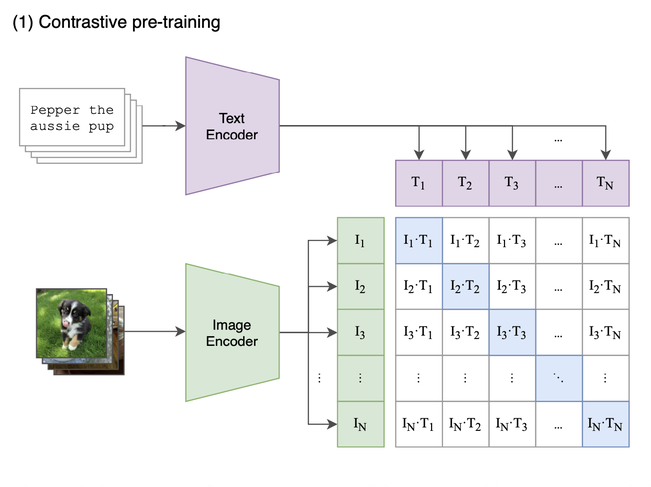
\includegraphics[width=0.62\textwidth]{images/2021-ICML-CLIP/fig-02.png}
\end{center}
\par\vspace{0.75em}\noindent{\zihao{4}\bfseries 2.2.1 预训练过程}\par\vspace{0.28em}
\begin{enumerate}
\item 输入：每个batch输入包含N个（image，text）pair。
\item 图像特征提取：每个image先经过\textbf{Image Encoder}抽取图像特征，得到图片的特征向量（i维）。
\item 文本特征提取：每个text经过\textbf{Text Encoder}抽取文本特征，得到文本的特征向量（t维）。
\item 投射层：上面图像、文本编码器提取的特征都要\textbf{通过矩阵乘法（简单的线性映射）映射到多模态空间}。
\begin{enumerate}
\item 图像特征通过一个线性变换映射到统一的\textbf{文本-图像多模态空间}，得到一个e维向量$I$。一个batch内所有N个image得到N个向量。
\item 文本特征通过一个线性变换映射到统一的\textbf{文本-图像多模态空间}，得到一个e维向量$T$。一个batch内所有N个text得到N个向量。
\end{enumerate}
\begin{feishuquote}
拿到图像的N个向量和文本的N个向量后就要开始对比学习了，让$I_1$配对$N_1$，一直到$I_N$配对$T_N$。\par
\end{feishuquote}
\item 正负样本构造：每个batch内所有的image和text\textbf{两两组合}可以得到$N*N$个（image，text）pair。其中，只有N组是正样本（对角线），其余$N*N-N$组是负样本（非对角线）。
\begin{feishuquote}
正负样本ground-truth定义：矩阵S中每个元素是一个image向量和一个text向量的内积相似度。S中\textbf{对角线上的元素是正样本，其余元素是负样本}。\par
\end{feishuquote}
\item 计算$N*N$个pair内部的相似度，得到的相似度用来做分类的logits。
\begin{feishuquote}
相似度计算采用余弦相似度（Cosine Similarity）：\par
一种用于衡量两个向量之间相似度的方法。它基于向量的余弦值，用于评估向量的方向和角度。余弦相似度的计算公式为：$\cos(s)=(a\cdot b)/(\|a\|\cdot \|b\|)$。\par
余弦相似度的值范围在-1到1之间，值越接近1，表示两个向量越相似；值越接近-1，表示两个向量越不相似；值为0时，表示两个向量相互垂直（正交）。\par
余弦相似度广泛应用于文本匹配、数据挖掘、机器学习等领域，用于评估样本之间的相似性。\par
在某些情况下，它可以替代欧氏距离，因为余弦相似度不仅考虑了向量的长度，还考虑了方向。\par
\end{feishuquote}
\item 训练loss定义：最大化正样本的相似性，最小化负样本的相似性。（对称式的目标函数，在对比学习中很常见。）logits 和 ground truth 的labels 计算交叉熵损失，$loss_i$、$loss_t$分别是 Image 和 Text 的 loss，最后求平均就得到loss。
预训练伪代码：\par
\begin{feishucode}
\begin{lstlisting}[language=clipnp]
'''
图像的输入I[n,h,w,c] ，文本的输入T[n,l]，其中n就是 batch size，l 是序列长度。
图像和文本的输入分别通过 Image Encoder 和 Text Encoder 得到图像和文本的特征I_f,T_f。
'''
I_f = image_encoder(I) #[n, d_i]
T_f = text_encoder(T) #[n, d_t]
'''
joint multimodal embedding [n, d_e]
在得到I_f和T_f后，这里还有一个投射层W_i, W_t
np.dot(I_f, W_i)将大小为_[n, d_i]的矩阵与大小为[d_i, d_e]的矩阵相乘，结果得到一个大小为[n, d_e]的投影矩阵
投射层主要就是学习如何从单模态变到多模态所以这是一个合并的多模态。
一个特征用来学习如何从单模态变成多模态，然后再做 L2 归一化，就得到了用来对比学习的特征I_e,T_e。
'''
I_e = l2_normalize(np.dot(I_f, W_i), axis=1)
T_e = l2_normalize(np.dot(T_f, W_t), axis=1)
'''
scaled pairwise cosine similarities [n, n]
有了n个图像的特征和n 个文本的特征之后，计算 cosine similarity，得到的相似度用来做分类的logits。
'''
logits = np.dot(I_e, T_e.T) * np.exp(t)
'''
symmetric loss function
这里的ground truth用的是arrange function生成，值从1开始1234567一直到n。
对于CLIP，它的正样本全在对角线上的，因此用这种方式创建ground truth。
'''
labels = np.arange(n)
'''
logits 和 ground truth 的labels 计算交叉熵损失
loss_i,loss_t分别是 Image 和 Text 的 loss，最后求平均就得到了loss。
'''
loss_i = cross_entropy_loss(logits, labels, axis=0)
loss_t = cross_entropy_loss(logits, labels, axis=1)
loss = (loss_i + loss_t)/2
\end{lstlisting}
\end{feishucode}
\end{enumerate}
\par\vspace{0.75em}\noindent{\zihao{4}\bfseries 2.2.2 模型结构}\par\vspace{0.28em}
CLIP是一个典型的双塔模型。有两个 encoder，一个对应图片，一个对应文本。\par
\begin{tcbraster}[raster columns=2, raster equal height=rows, raster column skip=9pt, raster row skip=8pt, raster left skip=0pt, raster right skip=0pt]
\begin{feishuboxnb}{callRedSoft}{💥}
Text Encoder\par
采用Transformer结构的变体GPT2。每条文本句子由[SOS]字符开始，[EOS]字符结束。GPT2最后一层[EOS]对应的向量作为整个文本的表征向量，就是后续用到的文本特征向量。\par
实验发现CLIP模型性能与文本抽取器的模型大小关系不是很大，所以当增加算力时，只增加text encoder的\textbf{宽度}，没有增加深度。\par
\end{feishuboxnb}
\begin{feishuboxnb}{callRedSoft}{📍}
Image Encoder\par
可以用ResNet、ViT等。ViT效果更好，默认采用ViT。\par
ViT使用CLS进行图像信息表征，CLS在\href{https://scnajei2ds6y.feishu.cn/wiki/QEJ8wXq9GiTBrxkMqbScnd8nnod}{ViT(2020, Google Research)}中即作为分类信息的表征。\par
\end{feishuboxnb}
\end{tcbraster}
\par\vspace{0.75em}\noindent{\zihao{4}\bfseries 2.2.3 训练细节}\par\vspace{0.28em}
\begin{itemize}
\item CLIP中的image encoder和text encoder都是从头开始训练的，没有使用微调方式，没有加载别的模型的参数进行初始化。
\begin{feishuquote}
why：\par
\begin{itemize}
\item CLIP 的训练目标是学习\textbf{图像-文本的多模态对齐关系}，而不是单纯的视觉或语言任务。
\item 如果使用 ImageNet 预训练的图像编码器，模型可能更偏向于\textbf{传统的分类任务，而非跨模态对齐}。
\item 从零开始训练可以确保模型不会受到单一模态（视觉或文本）的预训练偏见，而是能从一开始就学到\textbf{图像-文本之间的联合表示}。
\end{itemize}
\end{feishuquote}
\item 文本特征向量和图像特征向量，映射到多模态空间时，使用线性映射（乘以参数矩阵W），而没有使用非线性映射。
\item 数据增强只用随机裁剪。额外的数据增强会进一步增加计算开销，过强的数据增强可能会导致模型学习到与文本不匹配的视觉特征，影响图像-文本的对齐能力。
\item softmax的温度参数没有选作超参数，而是设置为一个可学习参数，在训练过程中联合优化。由于数据集太大，模型太大，计算量太大，不太好做超参数的选择。
\end{itemize}
\par\vspace{0.95em}\noindent{\zihao{3}\bfseries 2.3 推理阶段}\par\vspace{0.28em}
\begin{center}
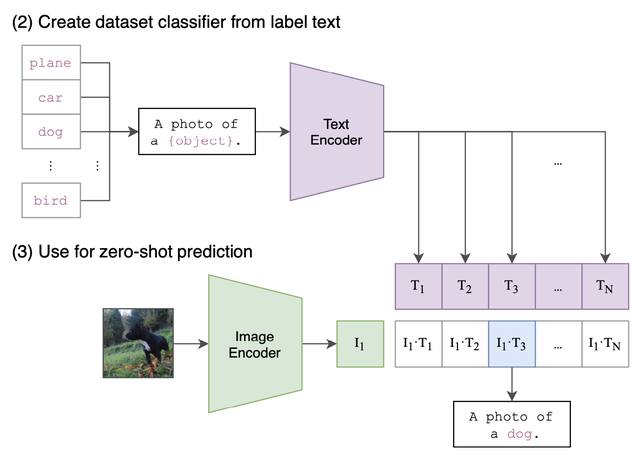
\includegraphics[width=0.62\textwidth]{images/2021-ICML-CLIP/fig-03.png}
\end{center}
这个阶段是使用 CLIP 的预训练好的 Image Encoder 和 Text Encoder 来做 Zero-Shot Transfer。比如来一张 ImageNet-1K 验证集的图片，我们希望 CLIP 预训练好的模型能完成这个分类的任务。\par
如下，CLIP采用了\textcolor{feishuRed}{\textbf{Prompt Template}}模式。\par
\par\vspace{0.75em}\noindent{\zihao{4}\bfseries 2.3.1 提取预测类别文本特征}\par\vspace{0.28em}
根据任务的分类标签构建每个类别的描述文本：A photo of \{label\}，然后将这些文本送入Text Encoder得到对应的文本特征，如果类别数目为N，那么将得到N个文本特征向量。\par
\begin{feishuquote}
以ImageNet为例，将所有类别的词汇 "cat"， "dog" 等, 做成一个 prompt: "A photo of a \{object\}", 并将这所有的prompt 输入到 CLIP 预训练好的 Text Encoder, 依次得到特征向量 $T_1, ..., T_N$\par
\end{feishuquote}
这些文本特征向量与图像的特征向量进行对比，这样，CLIP就可以将常见的分类任务转化为图文对比任务。\par
\par\vspace{0.75em}\noindent{\zihao{4}\bfseries 2.3.2 零样本预测（Zero-shot Prediction）}\par\vspace{0.28em}
将给定的图像送入Image Encoder得到图像特征，然后与N个文本特征进行对比，计算缩放的余弦相似度（和训练过程一致），选择相似度最大的文本对应的类别作为图像分类预测结果，进一步地，可以将这些相似度看成logits，送入softmax后可以到每个类别的预测概率。以此实现零样本分类。\par
\par\vspace{1.15em}\noindent{\zihao{-2}\bfseries 3. 总结}\par\vspace{0.28em}
CLIP的优势：CLIP将CNN中“相似的图片有相似的特征向量”往前推近了一大步，即不仅相似的图片有相似的特征向量，而且\textbf{相似的图片与文本也有相似的特征向量}。CLIP学习到的图片特征已经与人们描述这个视觉概念的自然语言产生了非常强的关系，它打通了文本和图片理解的界限，催生了后面多模态的无限可能。后续的“以图生文”，“以文搜图”都有赖这一点。\par
CLIP的局限：\par
\begin{itemize}
\item 图像-文本对齐有限
对比学习的方式\textbf{仅关注全局匹配}，而缺乏更细粒度的语义对齐\par
例：\par
它可以知道“一张猫的照片”对应一只猫的图像，但无法准确定位\textbf{猫在图像中的位置}。\par
如果一张图像中有\textbf{多个物体}，CLIP 可能无法准确地理解\textbf{哪些文本描述对应哪些局部区域}。\par
\item 文本理解能力不足
文本编码器是基于 \textbf{Transformer} 训练的，但它仅仅用于将文本转化为\textbf{固定维度的向量}，并没有对文本进行\textbf{深层理解，无法处理复杂的文本推理任务。}它无法结合多句描述进行上下文推理，而是单纯匹配文本与图像的相似度\par
例：\par
\begin{itemize}
\item “图中哪只狗看起来更开心？”
\item “这张图片的背景故事可能是什么？”
\end{itemize}
\item 难以处理细粒度分类
在\textbf{更细粒度的任务上（如区分相似物种、车型、品牌）表现较差}。在一些out-of-distribution数据集上也表现较差。\par
\item 对 Prompt 过于敏感
在推理时非常依赖Prompt Engineering，prompt微小的变化都会显著影响结果\par
例：对于同一张狗的图片，如果提供的文本是：\par
\begin{itemize}
\item “一只狗的照片（A photo of a dog）” → CLIP 可能能正确分类
\item “一只毛茸茸的宠物（A fluffy pet）” → CLIP 可能无法正确识别
\end{itemize}
\item 计算开销大，局部特征理解差
CLIP 主要处理全局图像信息，\textbf{对局部区域的理解较弱}\par
例：\par
一张图片里同时有“猫”和“狗”，但 CLIP 可能\textbf{无法清楚地定位这两个物体}，只能基于整体信息进行分类\par
\end{itemize}
\par\vspace{1.15em}\noindent{\zihao{-2}\bfseries 补充}\par\vspace{0.28em}
如何将GPT的思路（\textcolor{feishuBlue}{从互联网文本数据中通过自监督学习，}\textcolor{feishuBlue}{\textbf{自动提取监督信号}}\textcolor{feishuBlue}{，指导模型训练，从而能够实现广泛的可迁移性}）用到CV中，如何利用互联网上丰富多彩的图片、文本信息通过自监督的方式训练CV模型？\par
\begin{center}
\renewcommand{\arraystretch}{1.35}
\begin{tabularx}{\textwidth}{|>{\raggedright\arraybackslash}X|>{\raggedright\arraybackslash}X|}
\hline
\cellcolor{callYellow}\centering\arraybackslash \textcolor{feishuRed}{要解决的问题} & \cellcolor{cellLilac}\centering\arraybackslash \textcolor{feishuRed}{CLIP的做法} \\ \hline
\cellcolor{callGreen}如何构造文本-图片数据集\par 特点：充分利用互联网上已有信息。数据规模要大，内容要全，信息要广 & \cellcolor{callBlue}从互联网上挖掘了一个包含\textbf{4亿}个<image,text>对的数据集 \\ \hline
\cellcolor{callGreen}如何设计监督信号\par 特点：由于要大规模、自动化训练，没法依赖人工标注 & \cellcolor{callBlue}以预测图片和哪个文本是\textbf{成对出现}（因而具有语义相关性）作为训练目标。非常简单且巧妙地解决了如何从文本提取视觉监督信号的难题。 \\ \hline
\cellcolor{callGreen}如何设计大模型。\par 特点：模型容量要足够大，才能消费源源不断的数据源 & \cellcolor{callBlue}设计了包含Text encoder和image encoder并能联合训练的CLIP模型。通过当时主流的transformer和Resnet等解决模型容量问题。 \\ \hline
\cellcolor{callGreen}如何联合训练。\par 特点：文本-图片内容联合训练。 & \cellcolor{callBlue}具备超强的zero-shot迁移能力。以zero-shot的方式，无需微调，就能够在ImageNet数据集上取得和ResNet-50有监督训练一样的效果。这 \\ \hline
\end{tabularx}
\end{center}
\begin{feishubox}{callYellow}{🌟}
CLIP推理方法（\textbf{Prompt Template}）的优势：\par
摆脱了类别的限制。推理时遇到在训练数据集中没有出现的类别（例如“三轮车”）一样可以识别。只需在文本编码步骤加入“三轮车”的类别标签。\par
\textbf{prompt engineering：}将输入的标签转换成一个句子，例如"a photo of a \{label\}"。如果是在特定的类别上做推理，还可以加上一些额外的信息。例如，如果是宠物数据集，可以输入“a photo of a \{label\}, a type of pet”。再比如，对OCR数据集，可以在文本上增加双引号。通过增加额外信息，能够缩小解空间，提高效果。\par
\textbf{prompt ensembling：}对同一个label构造多个prompt template。通常是增加不同的形容词和修饰语。例如："a photo of a big \{label\}"、"a photo of a small \{label\}"。\par
\end{feishubox}
\par\vspace{1.15em}\noindent{\zihao{-2}\bfseries 代码}\par\vspace{0.28em}
整体调用代码\par
\begin{feishucode}
\begin{lstlisting}[language=Python]
# -------------------------- 整体调用示例 --------------------------

# -------------------------- CLIP核心类实现 --------------------------


# -------------------------- 图像编码器ViT实现 --------------------------

# -------------------------- 文本编码器实现 --------------------------


# -------------------------- 对比损失计算 --------------------------
\end{lstlisting}
\end{feishucode}
\begin{feishucode}
\begin{lstlisting}[language=Python]
import torch
from clip import clip
from PIL import Image

# 选择设备（优先GPU加速）
device = "cuda" if torch.cuda.is_available() else "cpu"
# 加载预训练模型（ViT-B/32是视觉transformer基础版，32是patch大小）
model, preprocess = clip.load("ViT-B/32", device=device)

# 图像预处理：调整尺寸/标准化等，并添加批次维度 → [1,3,224,224]
image = preprocess(Image.open("./CLIP.png")).unsqueeze(0).to(device)
# 文本预处理：将文字列表转换为token → [3,77]（3个文本，每个最多77个token）
text = clip.tokenize(["a diagram", "a dog", "a cat"]).to(device)

# 关闭梯度计算（推理模式）
with torch.no_grad():
    # 同时处理图像和文本，得到匹配分数矩阵
    # logits_per_image: 图片与各文本的相似度 → [1,3]
    # logits_per_text: 文本与各图片的相似度 → [3,1]
    logits_per_image, logits_per_text = model(image, text)
    
    # 对图片侧相似度做softmax得到概率分布
    probs = logits_per_image.softmax(dim=-1).cpu().numpy()

print("Label probs:", probs)  # 输出各标签概率，如[[0.99, 0.004, 0.003]]
\end{lstlisting}
\end{feishucode}
CLIP的实现\par
\begin{feishucode}
\begin{lstlisting}[language=Python]
class CLIP(nn.Module):
    def __init__(self,
                 embed_dim: int,          # 图文特征的统一维度（如512）
                 # 视觉部分参数
                 image_resolution: int,    # 输入图像尺寸（如224）
                 vision_layers: int,       # 视觉编码器层数（ViT的Transformer层数）
                 vision_width: int,        # 视觉编码器隐藏层维度（如768）
                 vision_patch_size: int,    # 图像分块大小（如32）
                 # 文本部分参数
                 context_length: int,      # 文本最大长度（如77个token）
                 vocab_size: int,          # 词表大小（如49408）
                 transformer_width: int,   # 文本编码器隐藏维度（如512）
                 transformer_heads: int,   # 文本多头注意力头数（如8）
                 transformer_layers: int   # 文本编码器层数（如12）
                 ):
        super().__init__()
        self.context_length = context_length  # 保存文本最大长度

        # 构建视觉编码器（ViT或ResNet二选一）
        if isinstance(vision_layers, (tuple, list)):
            # 使用改进版ResNet（当vision_layers是元组时）
            vision_heads = vision_width * 32 // 64  # 计算注意力头数
            self.visual = ModifiedResNet(...)       # 初始化ResNet结构
        else:
            # 使用Vision Transformer（默认）
            vision_heads = vision_width // 64       # 计算注意力头数
            self.visual = VisionTransformer(...)    # 初始化ViT结构

        # 构建文本编码器（Transformer结构）
        self.transformer = Transformer(...)
        
        # 文本嵌入相关参数
        self.token_embedding = nn.Embedding(vocab_size, transformer_width)  # 词嵌入层
        self.positional_embedding = nn.Parameter(...)  # 可学习位置编码
        self.ln_final = LayerNorm(transformer_width)   # 最终层归一化
        
        # 投影矩阵：将文本特征映射到统一空间
        self.text_projection = nn.Parameter(...)
        # 温度系数：控制相似度数值范围
        self.logit_scale = nn.Parameter(torch.ones([]) * np.log(1 / 0.07))
        
        self.initialize_parameters()  # 初始化权重

    def encode_image(self, image):
        # 视觉编码：输入图片 → 输出特征向量
        return self.visual(image.type(self.dtype))

    def encode_text(self, text):
        # 文本编码流程：
        x = self.token_embedding(text).type(self.dtype)  # 将token转为向量 [B,77,D]
        x += self.positional_embedding.type(self.dtype)  # 添加位置编码
        x = x.permute(1, 0, 2)  # 调整维度为[序列长度, 批次, 特征] → 适应Transformer
        x = self.transformer(x)  # 通过多层Transformer
        x = x.permute(1, 0, 2)  # 恢复维度为[批次, 序列, 特征]
        x = self.ln_final(x)     # 最终层归一化
        
        # 提取EOS（句子结束）位置的向量作为文本特征
        # text.argmax(dim=-1) 找到每个文本的实际长度（CLIP用最大id标记EOS）
        x = x[torch.arange(x.shape[0]), text.argmax(dim=-1)] 
        x = x @ self.text_projection  # 投影到统一特征空间
        return x

    def forward(self, image, text):
        # 获取图文特征（已归一化）
        image_features = self.encode_image(image)
        text_features = self.encode_text(text)
        
        # 归一化特征向量（使余弦相似度=点积）
        image_features = image_features / image_features.norm(dim=1, keepdim=True)
        text_features = text_features / text_features.norm(dim=1, keepdim=True)
        
        return image_features, text_features
\end{lstlisting}
\end{feishucode}
图像编码器ViT的实现\par
\begin{feishucode}
\begin{lstlisting}[language=Python]
class VisionTransformer(nn.Module):
    def __init__(self, input_resolution: int, patch_size: int, width: int, layers: int, heads: int, output_dim: int):
        super().__init__()
        self.input_resolution = input_resolution  # 输入尺寸（如224）
        self.patch_size = patch_size              # 分块大小（如32）
        
        # 分块卷积：将图像切分为32x32的块，每个块转为向量
        self.conv1 = nn.Conv2d(3, width, kernel_size=patch_size, stride=patch_size)
        
        # 可学习的类别标记（类似CLS token）
        scale = width ** -0.5  # 缩放因子（防止初始化过大）
        self.class_embedding = nn.Parameter(scale * torch.randn(width))
        
        # 位置编码：块数+1（例如(224/32)^2=49 → 49+1=50个位置）
        num_patches = (input_resolution // patch_size) ** 2
        self.positional_embedding = nn.Parameter(scale * torch.randn(num_patches + 1, width))
        
        # 预处理层归一化
        self.ln_pre = LayerNorm(width)
        
        # Transformer编码器堆叠
        self.transformer = Transformer(width, layers, heads)
        
        # 输出层归一化和投影矩阵
        self.ln_post = LayerNorm(width)
        self.proj = nn.Parameter(scale * torch.randn(width, output_dim))

    def forward(self, x: torch.Tensor):
        # 分块嵌入：输入[B,3,224,224] → [B,768,7,7]（假设width=768）
        x = self.conv1(x)
        
        # 展平：从[B,768,7,7] → [B,768,49] → 转置为[B,49,768]
        x = x.reshape(x.shape[0], x.shape[1], -1).permute(0, 2, 1)
        
        # 拼接类别标记：在序列开头添加可学习向量 → [B,50,768]
        class_embed = self.class_embedding.expand(x.shape[0], 1, -1)  # 扩展至批次大小
        x = torch.cat([class_embed, x], dim=1)
        
        # 添加位置编码 → [B,50,768]
        x += self.positional_embedding
        
        # 预处理层归一化
        x = self.ln_pre(x)
        
        # 通过Transformer（需调整维度为[序列长度, 批次, 特征]）
        x = x.permute(1, 0, 2)
        x = self.transformer(x)
        x = x.permute(1, 0, 2)
        
        # 取类别标记对应的特征 → [B,768]
        x = self.ln_post(x[:, 0, :])
        
        # 投影到统一特征空间 → [B,512]（假设output_dim=512）
        if self.proj is not None:
            x = x @ self.proj
        
        return x
\end{lstlisting}
\end{feishucode}
文本编码器的实现（在CLIP类中）\par
\begin{feishucode}
\begin{lstlisting}[language=Python]
def encode_text(self, text):
    # 文本编码流程：
    x = self.token_embedding(text).type(self.dtype)  # 将token转为向量 [B,77,D]
    x += self.positional_embedding.type(self.dtype)  # 添加位置编码
    x = x.permute(1, 0, 2)  # 调整维度为[序列长度, 批次, 特征] → 适应Transformer
    x = self.transformer(x)  # 通过多层Transformer
    x = x.permute(1, 0, 2)  # 恢复维度为[批次, 序列, 特征]
    x = self.ln_final(x)     # 最终层归一化
       
    # 提取EOS（句子结束）位置的向量作为文本特征
    # text.argmax(dim=-1) 找到每个文本的实际长度（CLIP用最大id标记EOS）
    x = x[torch.arange(x.shape[0]), text.argmax(dim=-1)] 
    x = x @ self.text_projection  # 投影到统一特征空间
return x
\end{lstlisting}
\end{feishucode}
其中文本 transformer 模块的实现如下：\par
\begin{feishucode}
\begin{lstlisting}[language=Python]
class Transformer(nn.Module):
    def __init__(self, width: int, layers: int, heads: int, attn_mask=None):
        super().__init__()
        # 堆叠多层Transformer块
        self.resblocks = nn.Sequential(*[
            ResidualAttentionBlock(width, heads, attn_mask) 
            for _ in range(layers)
        ])

    def forward(self, x: torch.Tensor):
        return self.resblocks(x)  # 顺序通过各层
\end{lstlisting}
\end{feishucode}
Loss\par
\begin{feishucode}
\begin{lstlisting}[language=Python]
def train():
    # 初始化CLIP模型
    model = CLIP(...)
    
    # 获取图文特征（已归一化）
    image_features, text_features = model(image, text)
    
    # 计算图文相似度矩阵（余弦相似度）
    logits = (text_features @ image_features.T)  # [B,B]
    
    # 计算图像间和文本间的自相似度（用于构造软目标）
    images_similarity = image_features @ image_features.T  # [B,B]
    texts_similarity = text_features @ text_features.T     # [B,B]
    
    # 构造目标分布（平均两种相似度）
    targets = F.softmax((images_similarity + texts_similarity) / 2, dim=-1)
    
    # 计算交叉熵损失（KL散度的简化形式）
    loss = (-targets * logits).sum(1).mean()
    return loss
\end{lstlisting}
\end{feishucode}

\end{document}
